\documentclass[aspectratio=169]{beamer}

% ─── Packages ─────────────────────────────────────────────────────────────────
\usepackage[T1]{fontenc}
\usepackage[utf8]{inputenc}
\usepackage{tikz}
\usepackage{xcolor}
\usepackage{array}
\usepackage{lmodern}

\usetikzlibrary{shapes.geometric, arrows.meta, positioning}

% ─── Colors ───────────────────────────────────────────────────────────────────
\definecolor{darkbg}{RGB}{15, 23, 42}
\definecolor{accent}{RGB}{99, 102, 241}
\definecolor{accentlight}{RGB}{165, 180, 252}
\definecolor{cardgray}{RGB}{30, 41, 59}
\definecolor{textgray}{RGB}{148, 163, 184}
\definecolor{successgreen}{RGB}{16, 185, 129}

% ─── Theme ────────────────────────────────────────────────────────────────────
\usetheme{default}
\setbeamertemplate{navigation symbols}{}
\setbeamertemplate{itemize item}{\color{accent}$\bullet$}
\setbeamertemplate{itemize subitem}{\color{accentlight}$\circ$}
\setbeamertemplate{enumerate item}{\color{accent}\textbf{\insertenumlabel.}}

\setbeamercolor{background canvas}{bg=darkbg}
\setbeamercolor{normal text}{fg=white}
\setbeamercolor{frametitle}{fg=accentlight, bg=cardgray}
\setbeamercolor{framesubtitle}{fg=textgray}
\setbeamercolor{structure}{fg=accent}
\setbeamercolor{block title}{fg=white, bg=accent}
\setbeamercolor{block body}{fg=white, bg=cardgray}
\setbeamercolor{alerted text}{fg=successgreen}
\setbeamercolor{itemize item}{fg=accent}
\setbeamercolor{enumerate item}{fg=accent}
\setbeamercolor{section in toc}{fg=accentlight}

\setbeamerfont{frametitle}{size=\large, series=\bfseries}
\setbeamerfont{title}{size=\Huge, series=\bfseries}

% ─── Footer ───────────────────────────────────────────────────────────────────
\setbeamertemplate{footline}{%
  \leavevmode%
  \hbox{%
    \begin{beamercolorbox}[wd=.5\paperwidth,ht=2.5ex,dp=1.125ex,left]{author in head/foot}%
      \hspace*{1em}\textcolor{textgray}{\small Briefly --- AI-Powered Meeting Intelligence}
    \end{beamercolorbox}%
    \begin{beamercolorbox}[wd=.5\paperwidth,ht=2.5ex,dp=1.125ex,right]{date in head/foot}%
      \textcolor{textgray}{\small \insertframenumber{} / \inserttotalframenumber}\hspace*{1em}
    \end{beamercolorbox}%
  }%
}

% ─── Helper ───────────────────────────────────────────────────────────────────
\newcommand{\hl}[1]{\textcolor{accentlight}{\textbf{#1}}}
\newcommand{\ok}[1]{\textcolor{successgreen}{\textbf{#1}}}
\newcommand{\acc}[1]{\textcolor{accent}{\textbf{#1}}}

% ─── Title ────────────────────────────────────────────────────────────────────
\title{\textbf{Briefly}}
\subtitle{AI-Powered Meeting Intelligence}
\author{Team Meeting Muse}
\date{\today}

% ══════════════════════════════════════════════════════════════════════════════
\begin{document}

% ─── Slide 1 : Title ──────────────────────────────────────────────────────────
\begin{frame}[plain]
  \begin{tikzpicture}[remember picture, overlay]
    \fill[cardgray, opacity=0.5]
      (current page.south west) rectangle (current page.north east);
    \draw[accent, line width=3pt]
      ([yshift=3pt]current page.south west) -- ([yshift=3pt]current page.south east);
  \end{tikzpicture}

  \vspace{1.5cm}
  \begin{center}
    {\fontsize{52}{60}\selectfont \textcolor{accentlight}{\textbf{Briefly}}}\\[0.4cm]
    \textcolor{accent}{\rule{9cm}{0.8pt}}\\[0.4cm]
    {\large \textcolor{textgray}{AI-Powered Meeting Intelligence}}\\[0.3cm]
    {\normalsize \textcolor{textgray}{Transcribe $\cdot$ Summarize $\cdot$ Act}}\\[0.8cm]
    {\small \textcolor{textgray}{Innovatex '26 Presentation --- \today}}
  \end{center}
\end{frame}

% ─── Slide 2 : The Problem ────────────────────────────────────────────────────
\begin{frame}{The Problem}
  \begin{columns}[T]
    \begin{column}{0.48\textwidth}
      \begin{block}{Meeting Overload}
        Professionals spend \hl{23 hrs/week} in meetings. Most insights are forgotten within 24 hours.
      \end{block}
      \vspace{0.3cm}
      \begin{block}{Lost Action Items}
        Teams lose track of \hl{40\% of action items} because no one has time to take proper notes.
      \end{block}
    \end{column}
    \begin{column}{0.48\textwidth}
      \begin{block}{Repetitive Catch-Ups}
        Team members who missed a meeting require costly \hl{catch-up calls}, creating endless meeting chains.
      \end{block}
      \vspace{0.3cm}
      \begin{block}{Language Barriers}
        Global teams struggle with non-native language meetings --- \hl{key context is lost} in translation.
      \end{block}
    \end{column}
  \end{columns}
\end{frame}

% ─── Slide 3 : Solution ───────────────────────────────────────────────────────
\begin{frame}{Our Solution --- Briefly}
  \centering
  \resizebox{\textwidth}{!}{%
  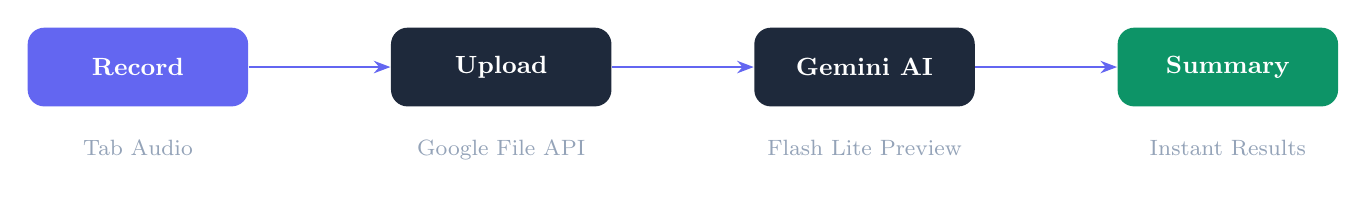
\begin{tikzpicture}[node distance=2cm, auto]
    \tikzstyle{box} = [rectangle, rounded corners=6pt, minimum width=2.8cm,
                       minimum height=1cm, text centered, text=white,
                       font=\small\bfseries, draw=none]
    \tikzstyle{arr} = [-{Stealth[length=6pt]}, thick, color=accent]

    \node[box, fill=accent]                        (rec)  {Record};
    \node[box, fill=cardgray, right=1.8cm of rec]  (up)   {Upload};
    \node[box, fill=cardgray, right=1.8cm of up]   (ai)   {Gemini AI};
    \node[box, fill=successgreen!80!black, right=1.8cm of ai] (out) {Summary};

    \draw[arr] (rec) -- (up);
    \draw[arr] (up)  -- (ai);
    \draw[arr] (ai)  -- (out);

    \node[below=0.3cm of rec, textgray, font=\footnotesize] {Tab Audio};
    \node[below=0.3cm of up,  textgray, font=\footnotesize] {Google File API};
    \node[below=0.3cm of ai,  textgray, font=\footnotesize] {Flash Lite Preview};
    \node[below=0.3cm of out, textgray, font=\footnotesize] {Instant Results};
  \end{tikzpicture}%
  }

  \vspace{0.7cm}
  \begin{columns}[c]
    \begin{column}{0.25\textwidth}
      \centering \ok{Transcript}\\\small Word-for-word record
    \end{column}
    \begin{column}{0.25\textwidth}
      \centering \ok{Action Items}\\\small Auto-extracted tasks
    \end{column}
    \begin{column}{0.25\textwidth}
      \centering \ok{Key Decisions}\\\small Important choices logged
    \end{column}
    \begin{column}{0.25\textwidth}
      \centering \ok{Diagrams}\\\small Auto Mermaid charts
    \end{column}
  \end{columns}
\end{frame}

% ─── Slide 4 : Key Features ───────────────────────────────────────────────────
\begin{frame}{Key Features}
  \begin{columns}[T]
    \begin{column}{0.48\textwidth}
      \begin{itemize}
        \item \hl{Reliable Audio Recording}\\
              \small Chrome \texttt{tabCapture} API --- no system muting
        \vspace{0.25cm}
        \item \hl{AI Transcription \& Summary}\\
              \small Gemini AI with smart model fallback
        \vspace{0.25cm}
        \item \hl{Multi-language Output}\\
              \small Results in any language your team needs
        \vspace{0.25cm}
        \item \hl{Mermaid Diagram Generation}\\
              \small Auto workflow charts from discussions
      \end{itemize}
    \end{column}
    \begin{column}{0.48\textwidth}
      \begin{itemize}
        \item \hl{Calendar Event Extraction}\\
              \small Deadlines and meetings auto-detected
        \vspace{0.25cm}
        \item \hl{Meeting Chat}\\
              \small Ask questions about any past meeting
        \vspace{0.25cm}
        \item \hl{Global Chat}\\
              \small Query across ALL your past meetings at once
        \vspace{0.25cm}
        \item \hl{Jira Ticket Generator}\\
              \small One click to create professional tickets
      \end{itemize}
    \end{column}
  \end{columns}
\end{frame}

% ─── Slide 5 : Tech Stack ─────────────────────────────────────────────────────
\begin{frame}{Tech Stack}
  \begin{columns}[T]
    \begin{column}{0.32\textwidth}
      \begin{block}{Frontend Extension}
        \begin{itemize}
          \item HTML5 \& CSS3
          \item Vanilla JavaScript
          \item Chrome MV3 API
          \item \texttt{chrome.sidePanel}
          \item \texttt{chrome.tabCapture}
          \item Web Audio API
        \end{itemize}
      \end{block}
    \end{column}
    \begin{column}{0.32\textwidth}
      \begin{block}{Backend API}
        \begin{itemize}
          \item Python 3
          \item FastAPI
          \item Uvicorn (ASGI)
          \item Pydantic v2
          \item python-dotenv
          \item CORS Middleware
        \end{itemize}
      \end{block}
    \end{column}
    \begin{column}{0.32\textwidth}
      \begin{block}{AI Layer}
        \begin{itemize}
          \item Google Gemini API
          \item \texttt{google-genai} SDK
          \item File Upload API
          \item Model fallback chain
          \item Auto-retry on 429/503
          \item JSON response mode
        \end{itemize}
      \end{block}
    \end{column}
  \end{columns}
\end{frame}

% ─── Slide 6 : Architecture ───────────────────────────────────────────────────
\begin{frame}{System Architecture}
  \centering
  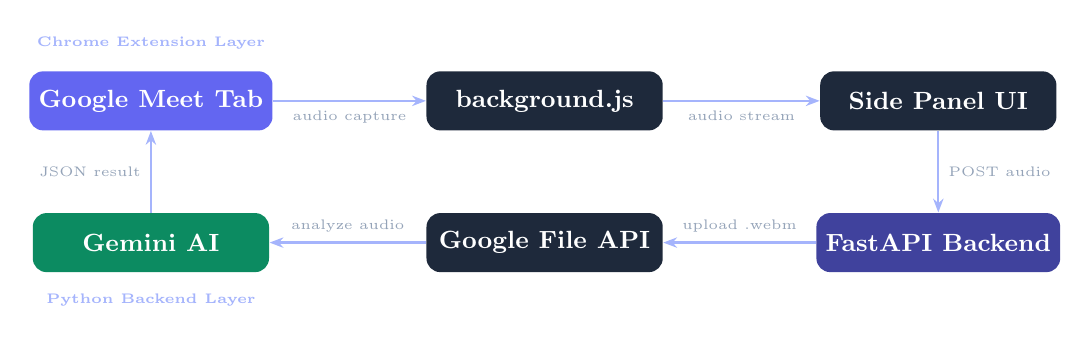
\begin{tikzpicture}[x=5cm, y=1.8cm, font=\small]
    \tikzstyle{box} = [rectangle, rounded corners=5pt,
                       minimum width=3cm, minimum height=0.75cm,
                       text centered, text=white, font=\small\bfseries, draw=none]
    \tikzstyle{arr} = [-{Stealth[length=5pt]}, thick, color=accentlight]
    \tikzstyle{lbl} = [font=\tiny, textgray]

    %% Column 0 (left), Column 1 (middle), Column 2 (right)
    %% Row 1 (top, y=1): L→R flow
    \node[box, fill=accent]              at (0,1) (meet) {Google Meet Tab};
    \node[box, fill=cardgray]            at (1,1) (bg)   {background.js};
    \node[box, fill=cardgray]            at (2,1) (sp)   {Side Panel UI};

    %% Row 2 (bottom, y=0): R→L flow (aligned under row 1)
    \node[box, fill=successgreen!75!black] at (0,0) (gem)  {Gemini AI};
    \node[box, fill=cardgray]              at (1,0) (gf)   {Google File API};
    \node[box, fill=accent!65!black]       at (2,0) (api)  {FastAPI Backend};

    %% ── Top row: left → right ──────────────────────────────────────────────
    \draw[arr] (meet.east) -- node[lbl, below]{audio capture} (bg.west);
    \draw[arr] (bg.east)   -- node[lbl, below]{audio stream}  (sp.west);

    %% ── Right side: Side Panel ↓ FastAPI (clean vertical) ─────────────────
    \draw[arr] (sp.south)  -- node[lbl, right]{POST audio} (api.north);

    %% ── Bottom row: right → left ───────────────────────────────────────────
    \draw[arr] (api.west)  -- node[lbl, above]{upload .webm}  (gf.east);
    \draw[arr] (gf.west)   -- node[lbl, above]{analyze audio} (gem.east);

    %% ── Left side: Gemini ↑ Google Meet (clean vertical, JSON result) ──────
    \draw[arr] (gem.north) -- node[lbl, left]{JSON result} (meet.south);

    %% ── Layer labels ───────────────────────────────────────────────────────
    \node[lbl, above=0.15cm of meet, font=\tiny\bfseries, accentlight]
      {Chrome Extension Layer};
    \node[lbl, below=0.15cm of gem, font=\tiny\bfseries, accentlight]
      {Python Backend Layer};
  \end{tikzpicture}
\end{frame}


% ─── Slide 7 : AI Resilience ──────────────────────────────────────────────────
\begin{frame}{AI Resilience Strategy}
  \begin{block}{3-Layer Fault Tolerance --- The backend never fails silently}
  \end{block}
  \vspace{0.5cm}
  \begin{columns}[T]
    \begin{column}{0.32\textwidth}
      \centering
      \textcolor{accent}{\Large $\blacksquare$}\\[0.2cm]
      \hl{Layer 1 --- Shield}\\[0.2cm]
      \small Auto-retries \textbf{3x} on \texttt{429}/\texttt{503} errors with exponential backoff (2\,s initial delay)
    \end{column}
    \begin{column}{0.32\textwidth}
      \centering
      \textcolor{accentlight}{\Large $\blacksquare$}\\[0.2cm]
      \hl{Layer 2 --- Safety Net}\\[0.2cm]
      \small If \texttt{gemini-3.1-flash-lite} fails, instantly retries with \texttt{gemini-2.5-flash} (no user impact)
    \end{column}
    \begin{column}{0.32\textwidth}
      \centering
      \textcolor{successgreen}{\Large $\blacksquare$}\\[0.2cm]
      \hl{Layer 3 --- Janitor}\\[0.2cm]
      \small \texttt{finally} block \textbf{always} deletes temp files from Google Cloud and local disk
    \end{column}
  \end{columns}
\end{frame}

% ─── Slide 8 : Demo ───────────────────────────────────────────────────────────
\begin{frame}{Live Demo}
  \begin{columns}[T]
    \begin{column}{0.55\textwidth}
      \textbf{\textcolor{accentlight}{Demo Flow:}}
      \vspace{0.3cm}
      \begin{enumerate}
        \item Open a \hl{Google Meet} tab
        \item Click the \hl{Briefly} icon --- Side Panel opens
        \item Click \ok{Start Recording}
        \item Speak naturally for 20--30 seconds
        \item Click \ok{Stop Recording}
        \item View instant \hl{AI Summary}:\\[0.15cm]
              \quad $\to$ Full Transcript\\
              \quad $\to$ Action Items\\
              \quad $\to$ Key Decisions\\
              \quad $\to$ Mermaid Diagram
        \item Try the \hl{Meeting Chat} feature!
      \end{enumerate}
    \end{column}
    \begin{column}{0.42\textwidth}
      \begin{block}{What Judges Will See}
        \begin{itemize}
          \item Real-time audio capture
          \item Zero-friction UX (side panel)
          \item Instant AI-generated output
          \item Graceful model fallback
          \item Clean, premium dark UI
        \end{itemize}
      \end{block}
    \end{column}
  \end{columns}
\end{frame}

% ─── Slide 9 : Future Scope ───────────────────────────────────────────────────
\begin{frame}{Future Scope}
  \begin{columns}[T]
    \begin{column}{0.48\textwidth}
      \begin{itemize}
        \item \hl{Cloud Sync}\\
              \small Access summaries from any device
        \vspace{0.25cm}
        \item \hl{Multi-user / Enterprise}\\
              \small Team dashboards and shared meeting notes
        \vspace{0.25cm}
        \item \hl{CRM Integration}\\
              \small Push action items to Salesforce, HubSpot
        \vspace{0.25cm}
        \item \hl{Zoom \& Teams Support}\\
              \small Extend beyond Google Meet
      \end{itemize}
    \end{column}
    \begin{column}{0.48\textwidth}
      \begin{itemize}
        \item \hl{Auto Email Summaries}\\
              \small Send notes to all participants automatically
        \vspace{0.25cm}
        \item \hl{Smart Notifications}\\
              \small Remind about upcoming action item deadlines
        \vspace{0.25cm}
        \item \hl{Analytics Dashboard}\\
              \small Meeting frequency and productivity insights
        \vspace{0.25cm}
        \item \hl{Mobile Companion App}\\
              \small View and search summaries on the go
      \end{itemize}
    \end{column}
  \end{columns}
\end{frame}

% ─── Slide 10 : Thank You ─────────────────────────────────────────────────────
\begin{frame}[plain]
  \begin{tikzpicture}[remember picture, overlay]
    \fill[cardgray, opacity=0.4]
      (current page.south west) rectangle (current page.north east);
    \draw[accent, line width=3pt]
      ([yshift=3pt]current page.south west) -- ([yshift=3pt]current page.south east);
  \end{tikzpicture}

  \vspace{1.2cm}
  \begin{center}
    {\fontsize{44}{52}\selectfont \textcolor{accentlight}{\textbf{Thank You!}}}\\[0.5cm]
    \textcolor{accent}{\rule{7cm}{0.8pt}}\\[0.5cm]
    {\Large \textcolor{white}{Questions?}}\\[0.8cm]
    {\normalsize \textcolor{textgray}{Built with Chrome MV3 $\cdot$ FastAPI $\cdot$ Google Gemini AI}}\\[0.5cm]
    {\small \textcolor{textgray}{\textit{``Briefly --- Never lose a meeting insight again.''}}}
  \end{center}
\end{frame}

\end{document}
